%%%%%%%%%%%%%%%%%%%%%%%%%%%%%%%%%%%%%%%%
% datoteka diploma-vzorec.tex
%
% vzorčna datoteka za pisanje diplomskega dela v formatu LaTeX
% na UL Fakulteti za računalništvo in informatiko
%
% vkup spravil Gašper Fijavž, december 2010
% 
%
%
% verzija 12. februar 2014 (besedilo teme, seznam kratic, popravki Gašper Fijavž)
% verzija 10. marec 2014 (redakcijski popravki Zoran Bosnić)
% verzija 11. marec 2014 (redakcijski popravki Gašper Fijavž)
% verzija 15. april 2014 (pdf/a 1b compliance, not really - just claiming, Damjan Cveta, Gašper Fijavž)

\documentclass[a4paper, 12pt]{book}

\usepackage[utf8x]{inputenc}   % omogoča uporabo slovenskih črk kodiranih v formatu UTF-8
\usepackage[slovene,english]{babel}    % naloži, med drugim, slovenske delilne vzorce
\usepackage[pdftex]{graphicx}  % omogoča vlaganje slik različnih formatov
\usepackage{fancyhdr}          % poskrbi, na primer, za glave strani
\usepackage{amssymb}           % dodatni simboli
\usepackage{amsmath}           % eqref, npr.
%\usepackage{hyperxmp}
\usepackage[pdftex, colorlinks=true,
						citecolor=black, filecolor=black, 
						linkcolor=black, urlcolor=black,
						pagebackref=false, 
						pdfproducer={LaTeX}, pdfcreator={LaTeX}, hidelinks]{hyperref}



%%%%%%%%%%%%%%%%%%%%%%%%%%%%%%%%%%%%%%%%
%	DIPLOMA INFO
%%%%%%%%%%%%%%%%%%%%%%%%%%%%%%%%%%%%%%%%
\newcommand{\ttitle}{Evalvacija čustev iz glasbe}
\newcommand{\ttitleEn}{Mood evaluation from music}
\newcommand{\tsubject}{\ttitle}
\newcommand{\tsubjectEn}{\ttitleEn}
\newcommand{\tauthor}{Primož Godec}
\newcommand{\tkeywords}{glasba, razpoloženje, evalvacija}
\newcommand{\tkeywordsEn}{music, mood, evaluation}



\usepackage{hyperref}
%%%%%%%%%%%%%%%%%%%%%%%%%%%%%%%%%%%%%%%%
%	HYPERREF SETUP
%%%%%%%%%%%%%%%%%%%%%%%%%%%%%%%%%%%%%%%%
\hypersetup{pdftitle={\ttitle}}
\hypersetup{pdfsubject=\ttitleEn}
\hypersetup{pdfauthor={\tauthor, p.godec9@gmail.com}}
\hypersetup{pdfkeywords=\tkeywordsEn}


 


%%%%%%%%%%%%%%%%%%%%%%%%%%%%%%%%%%%%%%%%
% postavitev strani
%%%%%%%%%%%%%%%%%%%%%%%%%%%%%%%%%%%%%%%%  
\renewcommand{\baselinestretch}{1.3} % ustrezen razmik med vrsticami
\setlength{\headheight}{15pt}        % potreben prostor na vrhu
\renewcommand{\chaptermark}[1]%
{\markboth{\MakeUppercase{\thechapter.\ #1}}{}} \renewcommand{\sectionmark}[1]%
{\markright{\MakeUppercase{\thesection.\ #1}}} \renewcommand{\headrulewidth}{0.5pt} \renewcommand{\footrulewidth}{0pt}
\fancyhf{}
\fancyhead[LE,RO]{\sl \thepage} \fancyhead[LO]{\sl \rightmark} \fancyhead[RE]{\sl \leftmark}



\newcommand{\BibTeX}{{\sc Bib}\TeX}

%%%%%%%%%%%%%%%%%%%%%%%%%%%%%%%%%%%%%%%%
% naslovi
%%%%%%%%%%%%%%%%%%%%%%%%%%%%%%%%%%%%%%%%  


\newcommand{\autfont}{\Large}
\newcommand{\titfont}{\LARGE\bf}
\newcommand{\clearemptydoublepage}{\newpage{\pagestyle{empty}\cleardoublepage}}
\setcounter{tocdepth}{1}	      % globina kazala

%%%%%%%%%%%%%%%%%%%%%%%%%%%%%%%%%%%%%%%%
% konstrukti
%%%%%%%%%%%%%%%%%%%%%%%%%%%%%%%%%%%%%%%%  
\newtheorem{izrek}{Izrek}[chapter]
\newtheorem{trditev}{Trditev}[izrek]
\newenvironment{dokaz}{\emph{Dokaz.}\ }{\hspace{\fill}{$\Box$}}

%%%%%%%%%%%%%%%%%%%%%%%%%%%%%%%%%%%%%%%%%%%%%%%%%%%%%%%%%%%%%%%%%%%%%%%%%%%%%%%
%% PDF-A
%%%%%%%%%%%%%%%%%%%%%%%%%%%%%%%%%%%%%%%%%%%%%%%%%%%%%%%%%%%%%%%%%%%%%%%%%%%%%%%

%%%%%%%%%%%%%%%%%%%%%%%%%%%%%%%%%%%%%%%% 
% define medatata
%%%%%%%%%%%%%%%%%%%%%%%%%%%%%%%%%%%%%%%% 
\def\Title{\ttitle}
\def\Author{\tauthor, p.godec9@gmail.com}
\def\Subject{\ttitleEn}
\def\Keywords{\tkeywordsEn}

%%%%%%%%%%%%%%%%%%%%%%%%%%%%%%%%%%%%%%%% 
% \convertDate converts D:20080419103507+02'00' to 2008-04-19T10:35:07+02:00
%%%%%%%%%%%%%%%%%%%%%%%%%%%%%%%%%%%%%%%% 
\def\convertDate{%
    \getYear
}

{\catcode`\D=12
 \gdef\getYear D:#1#2#3#4{\edef\xYear{#1#2#3#4}\getMonth}
}
\def\getMonth#1#2{\edef\xMonth{#1#2}\getDay}
\def\getDay#1#2{\edef\xDay{#1#2}\getHour}
\def\getHour#1#2{\edef\xHour{#1#2}\getMin}
\def\getMin#1#2{\edef\xMin{#1#2}\getSec}
\def\getSec#1#2{\edef\xSec{#1#2}\getTZh}
\def\getTZh +#1#2{\edef\xTZh{#1#2}\getTZm}
\def\getTZm '#1#2'{%
    \edef\xTZm{#1#2}%
    \edef\convDate{\xYear-\xMonth-\xDay T\xHour:\xMin:\xSec+\xTZh:\xTZm}%
}

\expandafter\convertDate\pdfcreationdate 

%%%%%%%%%%%%%%%%%%%%%%%%%%%%%%%%%%%%%%%%
% get pdftex version string
%%%%%%%%%%%%%%%%%%%%%%%%%%%%%%%%%%%%%%%% 
\newcount\countA
\countA=\pdftexversion
\advance \countA by -100
\def\pdftexVersionStr{pdfTeX-1.\the\countA.\pdftexrevision}


%%%%%%%%%%%%%%%%%%%%%%%%%%%%%%%%%%%%%%%%
% XMP data
%%%%%%%%%%%%%%%%%%%%%%%%%%%%%%%%%%%%%%%%  
\usepackage{xmpincl}
\includexmp{pdfa-1b}

%%%%%%%%%%%%%%%%%%%%%%%%%%%%%%%%%%%%%%%%
% pdfInfo
%%%%%%%%%%%%%%%%%%%%%%%%%%%%%%%%%%%%%%%%  
\pdfinfo{%
    /Title    (\ttitle)
    /Author   (\tauthor, damjan@cvetan.si)
    /Subject  (\ttitleEn)
    /Keywords (\tkeywordsEn)
    /ModDate  (\pdfcreationdate)
    /Trapped  /False
}


%%%%%%%%%%%%%%%%%%%%%%%%%%%%%%%%%%%%%%%%%%%%%%%%%%%%%%%%%%%%%%%%%%%%%%%%%%%%%%%
%%%%%%%%%%%%%%%%%%%%%%%%%%%%%%%%%%%%%%%%%%%%%%%%%%%%%%%%%%%%%%%%%%%%%%%%%%%%%%%

\begin{document}
\selectlanguage{slovene}
\frontmatter
\setcounter{page}{1} %
\renewcommand{\thepage}{}       % preprecimo težave s številkami strani v kazalu

%%%%%%%%%%%%%%%%%%%%%%%%%%%%%%%%%%%%%%%%
%naslovnica
%%%%%%%%%%%%%%%%%%%%%%%%%%%%%%%%%%%%%%%%
 \thispagestyle{empty}%
   \begin{center}
    {\large\sc Univerza v Ljubljani\\%
      Fakulteta za računalništvo in informatiko}%
    \vskip 10em%
    {\autfont \tauthor\par}%
    {\titfont \ttitle \par}%
    {\vskip 2em \textsc{DIPLOMSKO DELO\\[2mm]
    UNIVERZITETNI ŠTUDIJSKI PROGRAM PRVE STOPNJE RAČUNALNIŠTVO IN INFORMATIKA}\par}%
    \vfill\null%
    {\large \textsc{Mentor}: doc.\ dr. Matija Marolt\par}%
   
    {\vskip 2em \large Ljubljana 2014 \par}%
\end{center}
% prazna stran
\clearemptydoublepage

%%%%%%%%%%%%%%%%%%%%%%%%%%%%%%%%%%%%%%%%
%copyright stran
\thispagestyle{empty}
\vspace*{8cm}
{\small \noindent
Rezultati diplomskega dela so intelektualna lastnina avtorja.
Za objavljanje ali izkoriščanje rezultatov di\-plom\-ske\-ga dela je potrebno pisno soglasje avtorja, Fakultete za ra\-ču\-nal\-niš\-tvo in
informatiko ter mentorja%
\footnote{}


\begin{center}
\mbox{}\vfill
\emph{Besedilo je oblikovano z urejevalnikom besedil \LaTeX.}
\end{center}
% prazna stran
\clearemptydoublepage

%%%%%%%%%%%%%%%%%%%%%%%%%%%%%%%%%%%%%%%%
% stran 3 med uvodnimi listi
\thispagestyle{empty}
\vspace*{4cm}

\noindent
Fakulteta za računalništvo in informatiko izdaja naslednjo nalogo:
\medskip
\begin{tabbing}
\hspace{32mm}\= \hspace{6cm} \= \kill




Tematika naloge:
\end{tabbing}
Besedilo teme diplomskega dela študent prepiše iz študijskega informacijskega sistema, kamor ga je vnesel mentor. V nekaj stavkih bo opisal, kaj pričakuje od kandidatovega diplomskega dela. Kaj so cilji, kakšne metode uporabiti, morda bo zapisal tudi ključno literaturo.
\vspace{15mm}






\vspace{2cm}

% prazna stran
\clearemptydoublepage

%%%%%%%%%%%%%%%%%%%%%%%%%%%%%%%%%%%%%%%%
% izjava o avtorstvu
\vspace*{1cm}
\begin{center}
{\Large \textbf{\sc Izjava o avtorstvu diplomskega dela}}
\end{center}

\vspace{1cm}
\noindent Spodaj podpisani Primož Godec,
z vpisno številko \textbf{63110452}, sem avtor  diplomskega dela z naslovom:

\vspace{0.5cm}
\emph{Evalvacija čustev iz glasbe}

\vspace{1.5cm}
\noindent S svojim podpisom zagotavljam, da:
\begin{itemize}
	\item sem diplomsko delo izdelal samostojno pod mentorstvom
		doc.\ dr.\ Matije Marolta,

	\item	so elektronska oblika diplomskega dela, naslov (slov., angl.), povzetek (slov., angl.) ter ključne besede (slov., angl.) identični s tiskano obliko diplomskega dela,
	\item soglašam z javno objavo elektronske oblike diplomskega dela na svetovnem spletu preko univerzitetnega spletnega arhiva.	
\end{itemize}

\vspace{1cm}
\noindent V Ljubljani, dne 11. januarja 2011 \hfill Podpis avtorja:

% prazna stran
\clearemptydoublepage

%%%%%%%%%%%%%%%%%%%%%%%%%%%%%%%%%%%%%%%%
% zahvala
\thispagestyle{empty}\mbox{}\vfill\null\it%
Želim se zahvaliti mentorju Matiji Maroltu, za pomoč in spodbujanje pri raziskovanju in izdelavi diplomskega dela. Prav tako se želim zahvaliti Matevžu Pesku, ki si je vedno vzel čas, ko sem ga potreboval in s spodbujanjem poskrbel, da je bilo diplomsko delo napisano hitreje, kot bi bilo drugače. Zahvalil bi se tudi ekipi s katero smo sodelovali na projektu raziskovanja razpoloženja in glasbe. Ekipo sestavljajo Matevž Pesek, Matija Marolt, Mojca Poredoš, Jože Guna, Gregor Strle, Emilija Stojmenova in Matevž Pogačnik. Nazadnje bi se zahvalil še družini in prijateljem, ki mi vedno stojijo ob strani. 
\rm\normalfont

% prazna stran
\clearemptydoublepage

%%%%%%%%%%%%%%%%%%%%%%%%%%%%%%%%%%%%%%%%
% posvetilo
%%%%%%%%%%%%%%%%%%%%%%%%%%%%%%%%%%%%%%%%
\thispagestyle{empty}\mbox{}{\vskip0.20\textheight}\mbox{}\hfill\begin{minipage}{0.55\textwidth}%
...
\normalfont\end{minipage}

% prazna stran
\clearemptydoublepage

%%%%%%%%%%%%%%%%%%%%%%%%%%%%%%%%%%%%%%%%
% kazalo
\def\thepage{}% preprecimo tezave s stevilkami strani v kazalu
\tableofcontents{}


% prazna stran
\clearemptydoublepage

%%%%%%%%%%%%%%%%%%%%%%%%%%%%%%%%%%%%%%%%
% seznam kratic
%%%%%%%%%%%%%%%%%%%%%%%%%%%%%%%%%%%%%%%%

\chapter*{Seznam uporabljenih kratic}

\begin{tabular}{l|l|l}
  
  {\bf SVM} & support vector machine & metoda podpornih vektorjev \\
  \dots & \dots & \dots \\
\end{tabular}



% prazna stran
\clearemptydoublepage

%%%%%%%%%%%%%%%%%%%%%%%%%%%%%%%%%%%%%%%%
% povzetek
%%%%%%%%%%%%%%%%%%%%%%%%%%%%%%%%%%%%%%%
\addcontentsline{toc}{chapter}{Povzetek}
\chapter*{Povzetek}
V vzorcu je predstavljen postopek priprave diplomskega dela z uporabo okolja \LaTeX. Vaš povzetek mora sicer vsebovati približno 100 besed, ta tukaj je odločno prekratek.
\bigskip

\noindent\textbf{Ključne besede:} \tkeywords.
% prazna stran
\clearemptydoublepage

%%%%%%%%%%%%%%%%%%%%%%%%%%%%%%%%%%%%%%%%
% abstract
\selectlanguage{english}
\addcontentsline{toc}{chapter}{Abstract}
\chapter*{Abstract}
This sample document presents an approach to typesetting your BSc thesis using \LaTeX. A proper abstract should contain around 100 words which makes this one way too short.
\bigskip

\noindent\textbf{Keywords:} \tkeywordsEn.
\selectlanguage{slovene}
% prazna stran
\clearemptydoublepage

%%%%%%%%%%%%%%%%%%%%%%%%%%%%%%%%%%%%%%%%
\mainmatter
\setcounter{page}{1}
\pagestyle{fancy}

%%%%%%%%%%%%%%%%%%%%%%%%%%%%%%%%%%%%%%%
% UVOD
%%%%%%%%%%%%%%%%%%%%%%%%%%%%%%%%%%%%%%%

\chapter{Uvod}


\chapter{Pregled področja}


\chapter{Naš dataset}

Tema moje diplomske naloge je vsekakor evalvacija čustev iz glasbe s pomočjo računalnikih algoritmov. Dobre evalvacije pa ni možno narediti brez dobrega dataseta, zato smo se odločili, da zgradimo svoj dataset, ki bo osnova za raziskovanje povezave med čustvi in glasbo. Poleg tega smo se odločili, da datset nadgradimo s podatki o barvah, ki po mnenju anketirancev najbolje odražajo posamezno skladbo. Tako smo s tem pridoli še povzavo med čustvi, glasbo in barvami.

V naslednjih delih bom predstavil, kako smo zbirali podatke iz našega dataseta. Kasneje pa bom še analiziral nekatere podatke iz našega dataseta.

\section{Zbiranje dataseta}

Dataset smo zbirali s spletno anketo, ki smo jo sami implementirali. Še preden pa smo lahko naredili glavno anketo, smo morali sprejeti še nekaj odločitev, kako zgraditi anketo, da bo dala dobre in predvsem uporabne rezultate. Prva stvar, kjer je bil potreben premislek, je izbor oznak za emocije. Ugotovili smo, da obstajajo nekatere osnovne oznake za čustva, ki si jih je možno pogledati v \cite{dalgleish1999handbook}, ni pa standardnega seta oznak, ki bi se uporabljal na področju povezanem z razpoloženjem in glasbo. Nekatri avtorji so izbrali zbirko oznak čisto ituitivno naprimer \cite{wu2013spectral}. Zaradi tega smo se odločili, da naredimo prliminarno raziskavo v obliki ankete. 

\subsection{Preliminarna analiza}

Kot omenjeno smo preliminarno analizo izvajali s pomočjo ankete. To smo izvedli v elektronski obliki. V njej smo želeli preveriti osnovno strukturo glavne ankete, primernost elementov ankete in najbolj pomembno ugotoviti, katere oznake za čustva, so tista, ki bojo uporabljena v glavni anketi. Čustva smo izbirali tako, da je moral uporabnik za 46 oznak povedati, kako je neko čustvo prisotno pri njemu v tistem trenutku. Uporabnik je to označil na skali od 1 do 7. Iz tega seznama je bilo potem izbranih 17 osnovnih oznak uporabljenih v glavni anketi: aktivno, budno, dremavo, neaktivno, nesrečno, nezadovoljno, razočarano, sproščeno, srečno, utrujeno, vedro, veselo, zadovoljno, zaspano, žalostno, mirno in jezno.

slika skale

Kot sem že omenil nas je zanimala tudi struktura vprašalnika, ki je ostala približno enaka s to razliko, da smo v novem vprašalniku dodali del z glasbnenimi odseki ampak več o tem v [ref na chapter].

Poleg tega pa smo testirali tudi elemente uporabljene v anketi (7 stopenjska skala, neskončni barvni krog, izbira z radio gumbi in tekstovnimi polji). Ugotovili smo, da moramo nekatere elemente spremeniti. Najbolje smo spremenili barvno skalo, saj smo jo omejili na barvni krog z 49 možnostmi izbire. To je bilo potrebno, ker je imel na naeskončni skali uporabniki preveliko možnost izbiranja, obenem pa je bil sistem trodimenzionalen, kar večina uporabnikov sploh ni opazila in so nastavljali samo odtenek na svetlost pa so pozabili. Skala z 49 možnostmi (prikazana na sliki \ref{colorwheels}) se je izkazala kot odlična alternativa, saj še vedno ponuja veliko možnosti izbire barv, je prijazna uporabniku in pridobljeni podatki so boljši.

Poleg zamenjave barvnega kroga smo zamenjali tudi nekaj ostalih elementov. V delu, kjer uporabnik ozanči tri svoje najljubše žanre smo se odločili, da namesto vpisnih polj uporabniku ponudimo, da iz seznama izbere in na drug seznam potegne svojo izbiro. Za to smo se odločili, ker so uporabniki tja vpisovali tudi žanre, ki niso osnovni in tisti, ki sploh niso žanri. Prav tako nam je ta preliminarni vprašalnik pomagal izbrati kateri žanri so tisti, ki jih bomo uporabniku ponudili. Zamenjali smo še način, kako uporabnik vnese svoje trenutno razpoloženje in za ta namen uporabili nov element MoodGraph, ki ga bom opisal kasneje. 

\begin{figure}[ht]
\centering

\includegraphics[width=60mm]{colorwheelold.png}
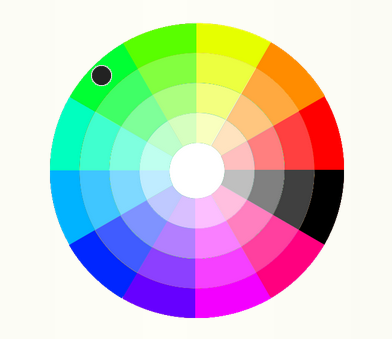
\includegraphics[width=60mm]{colorwheel.png}

\caption{Prvi barni krog smo v preliminarni anketi. V zunanjem krogu je bilo možno izbrati odtenek (hue) v notranjem pa je bilo možno izbirati nasičenost in svetlost. Drugi krog smo uporabili v glavni anketi. Imel je možnost izbire med 49 barvami. Rezina predstavljajo en barvni odtenek, proti notranjosti pa se spreminaja svetlost in intenzivnost. }
\label{colorwheels}
\end{figure}

\subsection{Glavna anketa}

Ko so bile izbrane oznake in struktura v grobem določena smo se lotili implementacije druge verzije vprašalnika, ki predstavlja glavni vprašalnik za zbiranje naše podatkovne zbirke. 

Glavni vprašalnik je bil sestavljen iz treh delov. V prvem delu smo spraševali po uporabnikovih demografskih podatkih, o poslušanju glasbe in glasbeni izobrazbi. V drugem delu nas je zanimalo predvsem uporabnikova percepcija razpoloženja, glasbe in barv. V tretjem delu so morali uporabniki ozačiti razpoloženje in barve v odlomku glasbe. 

\paragraph{Prvi del}

V tem delu smo spraševali o anketirančevi starosti, spolu in o tem ali živi na podeželju ali v mestu. Uporabnika smo vprašali tudi o tem ali je pod vplivom drog ali substanc. Zanimali so nas tudi podatki o glasbeni izobrazbi in o tem ali udeleženec igra inštrument ali poje. Poleg tega nas je še koliko časa dnevno uporabnik posluša glasbo. Anketrianec je moral tudi izbrati do tri svoje najljubše žanre in jih razporediti po priljubljenosti. To smo zajemal s pomočjo elementa prikazanega na sliki \ref{genresel}, kjer je uporabnik izmed seta 20 žanrov izbral najljubše in jih potegnil potegnil v stolpec desno ter razporedil po priljubljenosti. 

\begin{figure}[h!t]
\centering
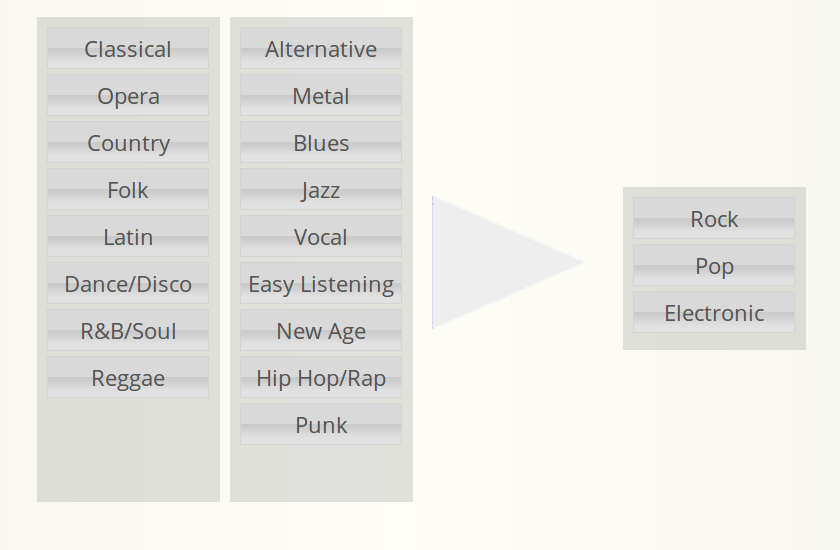
\includegraphics[width=10cm]{genresel.png}

\caption{Element v anketi uporabljen za izbiro najljubših žanrov}
\label{genresel}
\end{figure}

\paragraph{Drugi del}

Drugi del je namenjen zaznavanju anketirancovega trenutnega razpoloženja in njegove percepcije oznak za razpoloženje in barve za razpoloženje. To podatke zajemamo zato, ker na tak način lahko ugotovimo vzrok v različnih ocenah razpoloženja pri delu z glasbo. 

Na začetku je bil uporabnik vprašan kako bi svoje razpoloženje opisal s točko v prostoru, kjer zajemamo prijetnost in aktivnost (VA prostor) [ref]. To je dvodimenzionalen prostor, kjer na x osi od leve proti desni narašča prijetnost in od spodaj navzgor aktivnost.    Svoje razpoloženje je moral opisati tudi z izbiro barve s pomočjo elementa \ref{colorwheels}. 

Uporabnik je moral svoje razpoloženje opisati tudi z tem, da je povedal kako je posamezno čustvo pri nejm izraženo v trenutku reševanja ankete. To smo zajemali s pomočjo novega elementa imenovanega MoodStripe. Potrebno je bilo potegniti posamezne oznake čustev v prostor, kjer od leve proti desni narašča prisotnost posamznega čustva. Če je anketiranec postavil čustvo skrajno levo to pomeni, da to čustvo pri njem ni prisotno, če pa ga je posavil skrajno desno to pomeni, da je čustvo zelo prisotno 

\begin{figure}[ht]
\centering
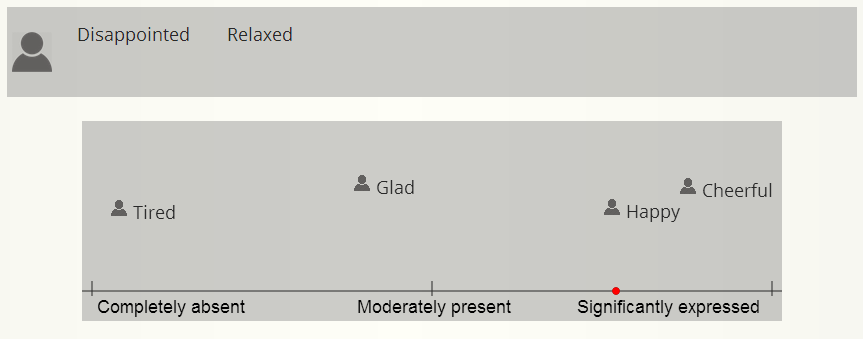
\includegraphics[width=10cm]{moodstripe.png}

\caption{Element za zajemanje pristnosti posameznega čustva imenovan moodstripe.}
\label{genresel}
\end{figure}

V drugem delu smo uporabnika povprašali tudi o njegovi percepciji posameznega čustva. Anketiranec je moral za vsako čustveno oznako povedati kako prijetno je to čustvo in kako aktivno je (VA vrednost). To smo zajemali s pomočjo elementa imenovanega enokategorni MoodGraph (slika \ref{moodgraph}). To je 2D prostor, kjer je na vodoravni osi prijetnost in na navpični osi anktivnost. Uporabnik je ozake čustev prikazane nad grafom potegnil v to ravnino na mesto za katerega misli, da ga najbolje opisuje. 

\begin{figure}[ht]
\centering
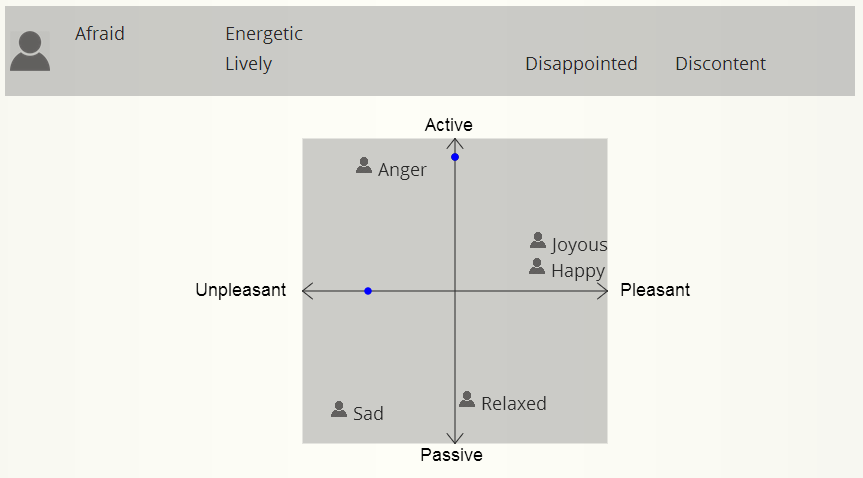
\includegraphics[width=10cm]{images/moodgraph.png}

\caption{}
\label{moodgraph}
\end{figure}

Poleg tega kako si uporabnik predstavlja posamezno čustvo v VA prostoru nas je zanimalo tudi kako bi uporabniku opisal ista čustva z barvno. To smo izvedli s pomočjo barvnega krogra (slika \ref{colorwheels}), ki sem ga že opisal zgoraj. 

\paragraph{Tretji del}

V tretjem delu smo vprašali anketirance, da ozačijo 10 glasbenih odlomkov dolgih 15 sekund. Odlomki so bili izbrani iz nabora 200 odlomkov. Glasba je bila izbrana tako, da je bila uporabnikom nepoznana. S tem smo se izognili pristranskosti zaradi uporabnikovega poznavanja določene glasbe in vpliva dogodkov, ki so se mu zgodili ob poslušanju določene pesmi. Vsak uporabnik je dobil samo 10 odlomkov iz tega razloga, da uporabnikov nebi preveč obremenili in bi zaradi tega dobili slabše ocene. 

Glasba je bila izbrana iz 4 različnih virov. 80 pesmi smo izbrali iz odprte podatkovne zbirke Jamendo. Iz tega vira smo izbrali bolj vsakdanjo glasbo različnih zvrsti. Naslednjih 80 pesmi smo vzeli iz zbirke filmske glasbe opisane v \cite{eerola2010comparison}. Dodali smo še 20 slovenskih etno pesmi in 20 pesmi iz nabora moderne elektro-akustične glasbe. 

Za vsak odlomek je moral uporanik narediti dve stvari. Najprej je s pomočjo barvnega kroga (slika \ref{colorwheels}) povedal s katero barvo bi opisal posamezno pesem. Nato pa je v drugem koraku izbral katera čustva so izražena v odlomku in katera čustva posamezna glasba vzbudi pri njem. Za prvo je izbiral izmed nabora 14 oznak, za drugo pa je iz nabora 10 ozank. Poleg tega, da je izbral posamezno oznako jo je moral še uvrstiti v VA prostor. S tem smo zajeli tudi podatek kako si predstavlaja določeno oznako pri posamezni pesmi. Naprimer pri neki pesmi je lahko veselje zelo aktivno, pri drugi pa majn. Poleg tega nam ta podatek da možnost, da raziskujemo tudi samo kako si uporabnik v VA prostoru predstavlja posamezno pesem. Za zajemanje tega podatka smo uporabili dvokategorni MoodGraph prikazan na sliki \ref{moodgraphdvo}.

\begin{figure}[ht]
\centering
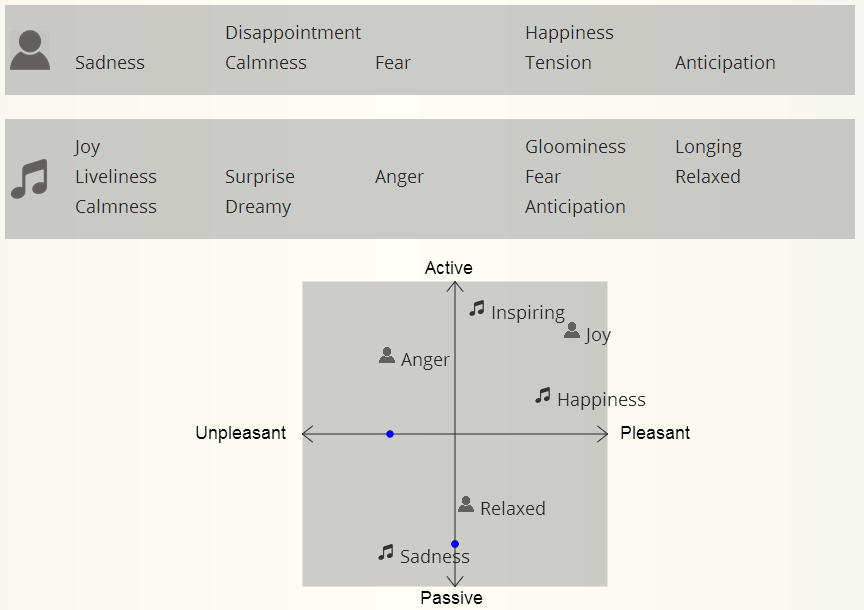
\includegraphics[width=10cm]{images/moodgraphdvo.png}

\caption{}
\label{moodgraphdvo}
\end{figure}

\subsection{Evaluacijska anketa}

\section{Sestava datasta}

Z zgoraj opisano anketo smo zbrali dataset 




\bibliography{diploma}{}
\bibliographystyle{plain}

\end{document}

